%%%%%%%%%%%%%%%%%%%%%%%%%%%%%%%%%%%%%%%%%%%%%%%%%%%%%%%%%%%%%%%%%%%%%%%%%%%%%%%%%%
\begin{frame}[fragile]\frametitle{}
\begin{center}
{\Large Consulting}

{\tiny (Ref: Leadership needs us to do Gen AI, what do we do? - Chip Huyen)}

\end{center}
\end{frame}


%%%%%%%%%%%%%%%%%%%%%%%%%%%%%%%%%%%%%%%%%%%%%%%%%%%%%%%%%%%
\begin{frame}[fragile]\frametitle{Phase 1: Exploration}

\begin{itemize}
\item Set expectations
\item Minimize risks
\item Invest in things that last
\item Experiment
\end{itemize}	

\end{frame}


%%%%%%%%%%%%%%%%%%%%%%%%%%%%%%%%%%%%%%%%%%%%%%%%%%%%%%%%%%%
\begin{frame}[fragile]\frametitle{Set expectations}

\begin{itemize}
\item Building some cool demos with LLMs : Easy
\item Actually building a product with LLMs : Hard
\item If you just want some cool demos to show customers that you’re ahead of the 
curve, go for it.
\item If you just want your team to experiment and build out LLM muscle, go for it.
\item If you want a product, set goals for what you expect that product will bring, and the 
resources you’re willing to invest.
\end{itemize}	

\end{frame}

%%%%%%%%%%%%%%%%%%%%%%%%%%%%%%%%%%%%%%%%%%%%%%%%%%%%%%%%%%%
\begin{frame}[fragile]\frametitle{There are a lot of things LLMs can do}

\begin{itemize}
\item Q: But can these things meaningfully transform your business?
\item A: Unclear
\end{itemize}	

\end{frame}


%%%%%%%%%%%%%%%%%%%%%%%%%%%%%%%%%%%%%%%%%%%%%%%%%%%%%%%%%%%
\begin{frame}[fragile]\frametitle{There are a lot of things LLMs can’t do NOW}

\begin{itemize}
\item Q: But would LLMs still not able to do those in the future?
\item A: Unclear
\end{itemize}	


“When a distinguished but elderly scientist states that something is possible, he is almost 
certainly right. When he states that something is impossible, he is very probably wrong.”
- Arthur Clarke

\end{frame}


%%%%%%%%%%%%%%%%%%%%%%%%%%%%%%%%%%%%%%%%%%%%%%%%%%%%%%%%%%%
\begin{frame}[fragile]\frametitle{We live in an era of changes and uncertainty}

In times of uncertainty, apply a decision-making framework to minimize regrets

Minimize risks:
\begin{itemize}
\item Evaluate how disruptive gen AI is to your business
\item Figure out your data story
\item Avoid big, sweeping decisions
\end{itemize}	

\end{frame}

%%%%%%%%%%%%%%%%%%%%%%%%%%%%%%%%%%%%%%%%%%%%%%%%%%%%%%%%%%%
\begin{frame}[fragile]\frametitle{Evaluate how disruptive gen AI is to your business}

\begin{itemize}
\item If I don’t do anything, can competitors with gen AI make me obsolete?
	\begin{itemize}
		\item Creative work: advertising, design, gaming, media, entertainment
		\item A lot of document processing: legal, insurance, HR
	\end{itemize}	
		
		Go all in
\item If I don’t do anything, will I miss out opportunities to boost revenue?
	\begin{itemize}
		\item Customer support: chat, call centers
		\item Search \& recommendation
		\item Productivity enhancement: automated note-taking, summarization, information aggregation
	\end{itemize}	
	
	Build vs Buy decision

\item If there are opportunities, what advantages do I have to capture them?
	\begin{itemize}
		\item Proprietary data
		\item A100s lying around
		\item Existing user base
	\end{itemize}	
		
	Make bets
\end{itemize}	

\end{frame}

%%%%%%%%%%%%%%%%%%%%%%%%%%%%%%%%%%%%%%%%%%%%%%%%%%%%%%%%%%%
\begin{frame}[fragile]\frametitle{Figure out your data story}

\begin{itemize}
\item Consolidate existing data across departments and sources
\item Update your data terms of use 
\item Put guardrails around data quality + governance
\end{itemize}	

\end{frame}

%%%%%%%%%%%%%%%%%%%%%%%%%%%%%%%%%%%%%%%%%%%%%%%%%%%%%%%%%%%
\begin{frame}[fragile]\frametitle{Avoid big, sweeping decisions}

\begin{itemize}
\item “Stop everything to figure out our generative AI.”
\item “Let’s buy as many A100s as we can.”
\end{itemize}	

It’s okay to make big bets as long as you can back them up with evidence.
\end{frame}

%%%%%%%%%%%%%%%%%%%%%%%%%%%%%%%%%%%%%%%%%%%%%%%%%%%%%%%%%%%
\begin{frame}[fragile]\frametitle{Invest in things that last}

The future life expectancy of some non-perishable things, like a technology or an 
idea, is proportional to their current age
- Lindy’s Law
\end{frame}

%%%%%%%%%%%%%%%%%%%%%%%%%%%%%%%%%%%%%%%%%%%%%%%%%%%%%%%%%%%
\begin{frame}[fragile]\frametitle{LLM fundamentals have been around for a while}

\begin{itemize}
\item Language modeling (1951)
\item Embeddings (2003)
\item Vector databases: Facebook’s Faiss (2017), Google’s ScaNN (2020)
\item Making data faster, cheaper, more accessible will always be important
\end{itemize}	

\end{frame}

%%%%%%%%%%%%%%%%%%%%%%%%%%%%%%%%%%%%%%%%%%%%%%%%%%%%%%%%%%%
\begin{frame}[fragile]\frametitle{Personal litmus test}

\begin{itemize}
\item Does this seem hacky to me?
\item Context learning vs. prompt engineering
\end{itemize}	

\end{frame}

%%%%%%%%%%%%%%%%%%%%%%%%%%%%%%%%%%%%%%%%%%%%%%%%%%%%%%%%%%%
\begin{frame}[fragile]\frametitle{Model architectures, tools, techniques will certainly evolve}

AI literacy will be less about how to build a transformer model from scratch, and 
more about how to use AI appropriately

\end{frame}

%%%%%%%%%%%%%%%%%%%%%%%%%%%%%%%%%%%%%%%%%%%%%%%%%%%%%%%%%%%
\begin{frame}[fragile]\frametitle{Experiment}

\begin{itemize}
\item Timebox your experiment
\item Clarify the decisions you want to make by the end
\item APIs are cheap and easy for experiment: \$100 and one weekend can take you a long way!!
\end{itemize}	

\end{frame}

%%%%%%%%%%%%%%%%%%%%%%%%%%%%%%%%%%%%%%%%%%%%%%%%%%%%%%%%%%%
\begin{frame}[fragile]\frametitle{Understand LLM behaviors (dealbreakers??)}

\begin{itemize}
\item Ambiguous inputs + outputs
\item Hallucination vs. factuality
\item Privacy: how to ensure LLMs don’t reveal your user PII info?
\item Unstable infra: performance + latency
\item Inference cost
\item Forward \& backward compatibility
\end{itemize}	

\end{frame}

%%%%%%%%%%%%%%%%%%%%%%%%%%%%%%%%%%%%%%%%%%%%%%%%%%%%%%%%%%%
\begin{frame}[fragile]\frametitle{Phase 2: Building}

\begin{itemize}
\item Understand the LLM stack
\item Implement:
	\begin{itemize}
	\item Gather data
	\item Choose a model
	\item Get the most out of each layer of the stack before moving to the next
	\end{itemize}	
\item Evaluate
\end{itemize}	

\end{frame}

%%%%%%%%%%%%%%%%%%%%%%%%%%%%%%%%%%%%%%%%%%%%%%%%%%%%%%%%%%%
\begin{frame}[fragile]\frametitle{The LLM stack}

\begin{itemize}
\item LLM part
	\begin{itemize}
	\item Prompt engineering
	\item Fine-tuning, distillation
	\item Training a model from scratch
	\end{itemize}	
\item Infra around LLM
	\begin{itemize}
	\item Databases
	\item Logs
	\item Caching
	\end{itemize}
\end{itemize}	

\end{frame}

%%%%%%%%%%%%%%%%%%%%%%%%%%%%%%%%%%%%%%%%%%%%%%%%%%%%%%%%%%%
\begin{frame}[fragile]\frametitle{Work-flow}

\begin{center}
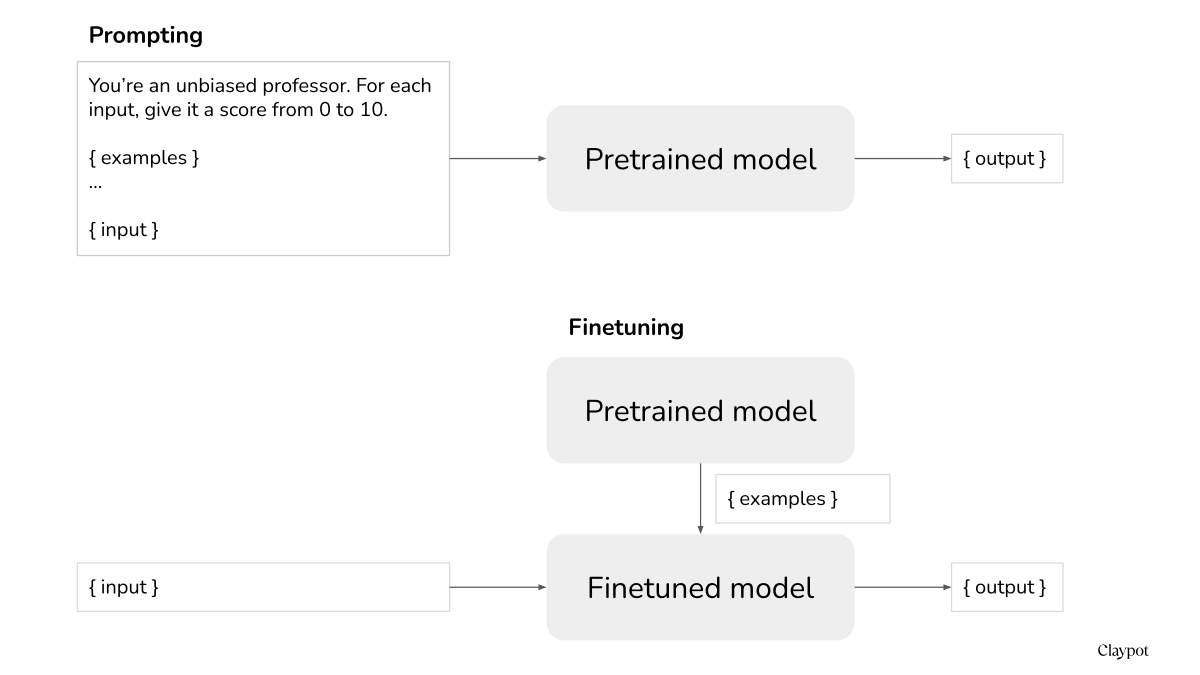
\includegraphics[width=\linewidth,keepaspectratio]{llm43}

{\tiny (Ref: Leadership needs us to do Gen AI, what do we do? - Chip Huyen)}
\end{center}
\end{frame}

%%%%%%%%%%%%%%%%%%%%%%%%%%%%%%%%%%%%%%%%%%%%%%%%%%%%%%%%%%%
\begin{frame}[fragile]\frametitle{Work-flow}

\begin{center}
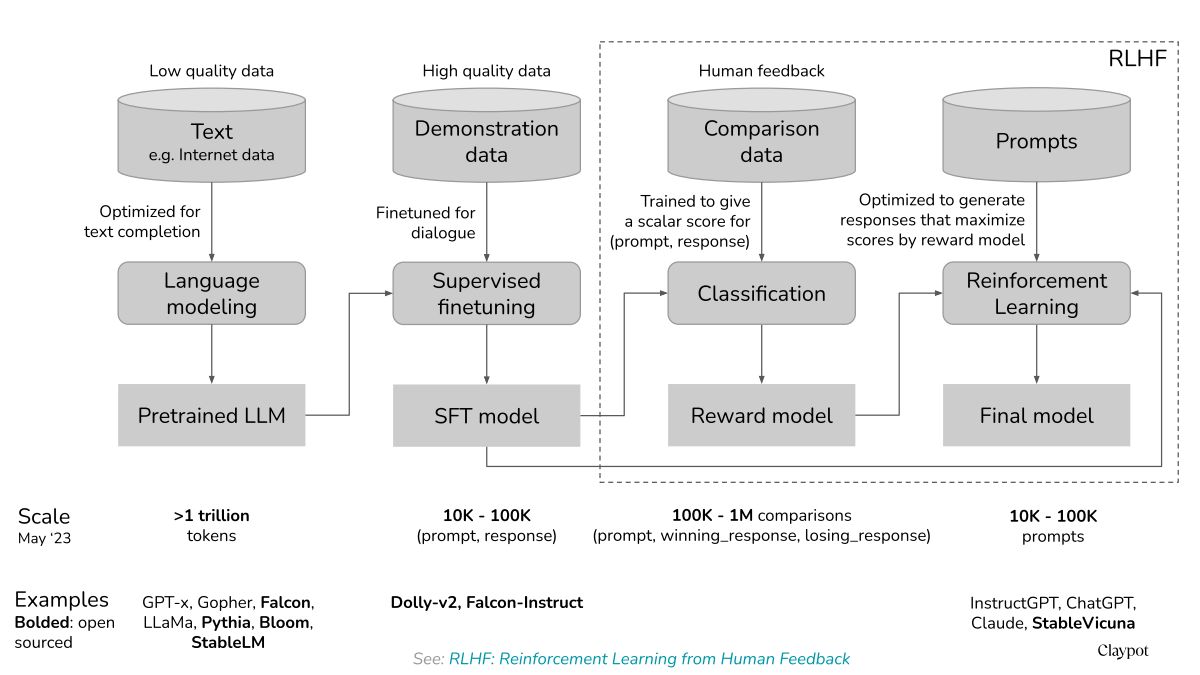
\includegraphics[width=\linewidth,keepaspectratio]{llm44}

{\tiny (Ref: Leadership needs us to do Gen AI, what do we do? - Chip Huyen)}
\end{center}
\end{frame}

%%%%%%%%%%%%%%%%%%%%%%%%%%%%%%%%%%%%%%%%%%%%%%%%%%%%%%%%%%%
\begin{frame}[fragile]\frametitle{Work-flow}

\begin{center}
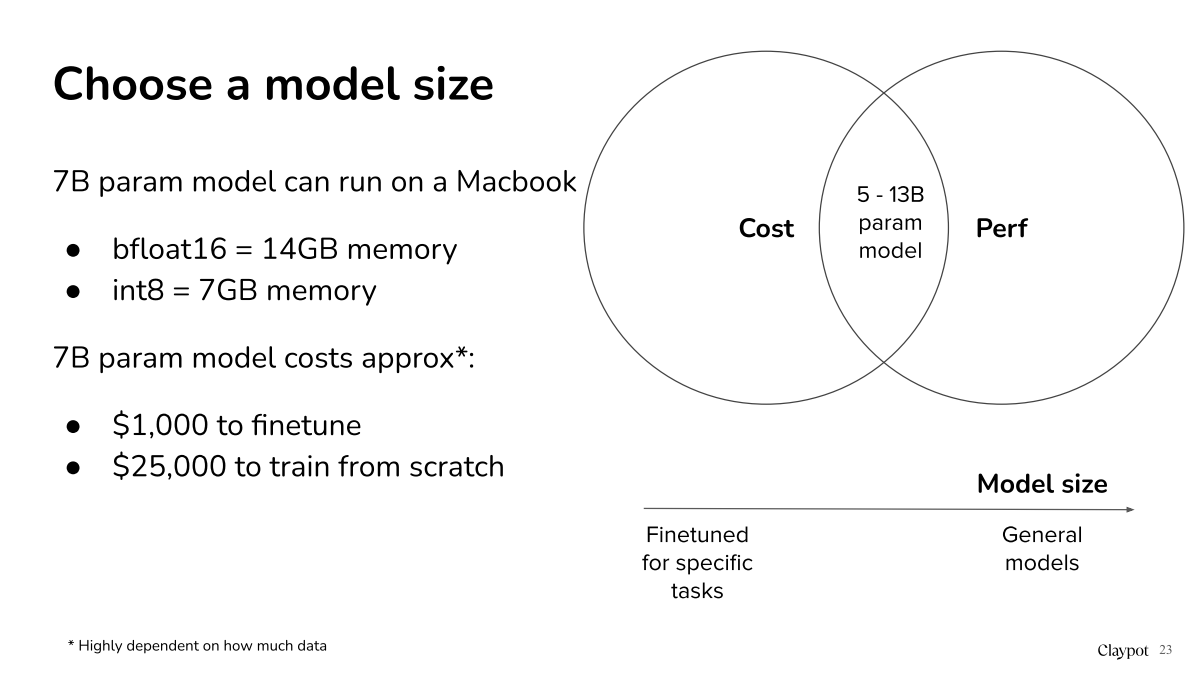
\includegraphics[width=\linewidth,keepaspectratio]{llm45}

{\tiny (Ref: Leadership needs us to do Gen AI, what do we do? - Chip Huyen)}
\end{center}
\end{frame}

%%%%%%%%%%%%%%%%%%%%%%%%%%%%%%%%%%%%%%%%%%%%%%%%%%%%%%%%%%%
\begin{frame}[fragile]\frametitle{Evaluate}

\begin{itemize}
\item Tie to your OWN business metrics
\item Build your own test set
\item Beware of standardized evaluation: still catching up with use cases
\end{itemize}	

\end{frame}

%%%%%%%%%%%%%%%%%%%%%%%%%%%%%%%%%%%%%%%%%%%%%%%%%%%%%%%%%%%
\begin{frame}[fragile]\frametitle{Takeaways}

\begin{itemize}
\item Set concrete goals
\item Data story is more important now than ever
\item Invest in things that last
\item Experiment with APIs, build with open-source
\item Understanding LLM behaviors: which is a dealbreaker for your use case?
\item Choose a model size that balances between cost and performance
\item Always tie model evaluation to your business metrics
\item Have fun!
\end{itemize}	

\end{frame}